We are requested to design a Private Mobile Radio (PMR) Network working at VHF
frequencies.
\begin{figure}[H]
    \centering
    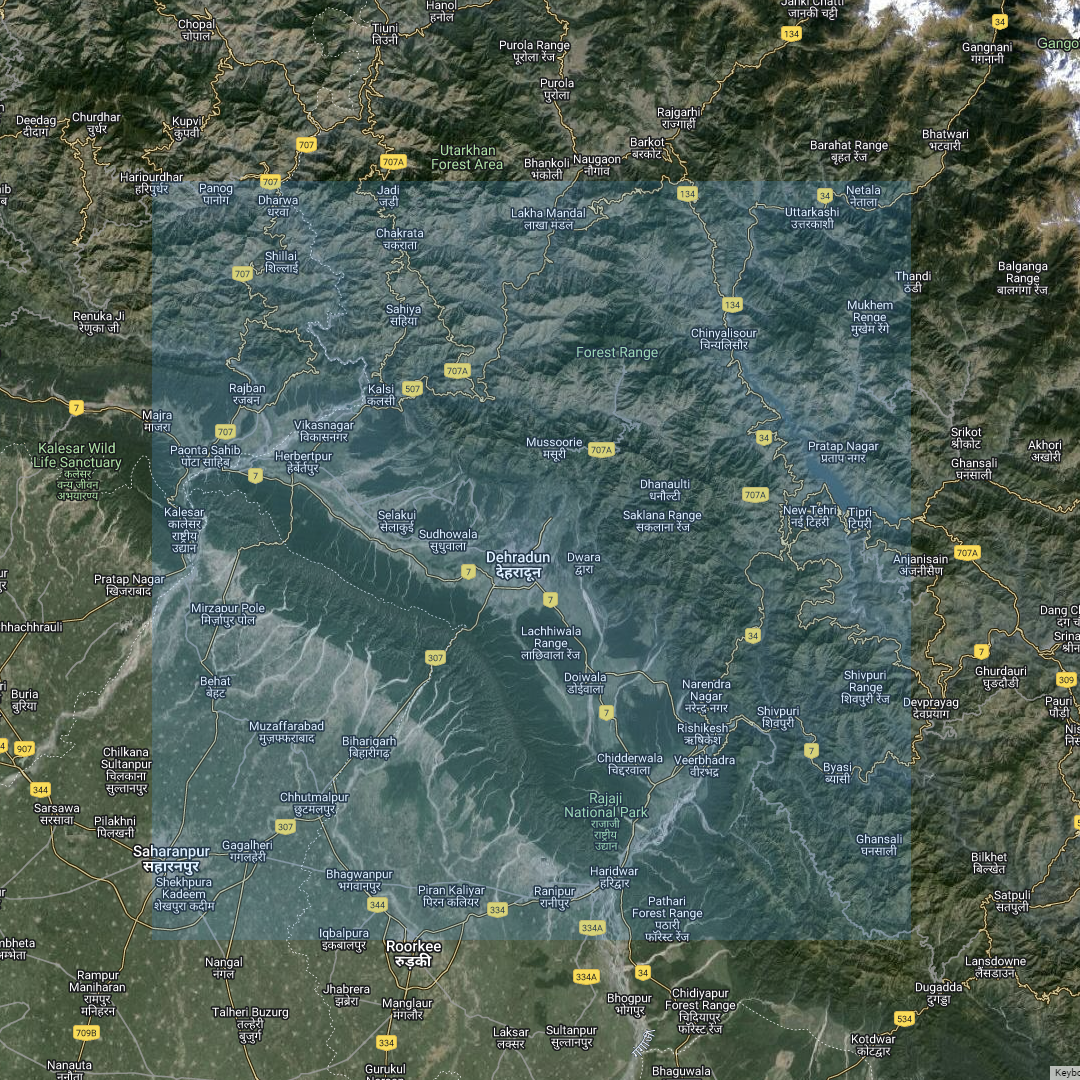
\includegraphics[width = 0.6\textwidth]{Images/Area of interest.png}
    \caption{Area of interest - \textit{Dehradun, India}}
    \label{fig:enter-label}
\end{figure}

Specifications of the radio network are:
\begin{itemize}
\item Covered region: a 100 km $\times$ 100 km square area centered around the city of
Dehradun, India (the centre of the area of interest, with coordinates 30$^\circ$ 20' 42" N, 78$^\circ$ 1' 44.4" E is shown in the attached map above)
\item Frequency of operation: 163 MHz
\item Modulation type: ETSI Digital Mobile Radio (DMR)
\item Repeaters’ interconnection: point-to-point microwave links at 28 GHz
\item Repeater stations (DMR): Motorola SLR5500\cite{MotorolaSLR5500}.
\begin{itemize}
    \item RF Output Power: 1-50 W
    \item Sensitivity (typical): 0,22 $\mu$V 
\end{itemize}
\item Vehicular terminals (DMR): Motorola DM4000e\cite{MotorolaDME4000E}.
\begin{itemize}
    \item Digital Sensitivity (5\% BER) : 0.16 $\mu$V
    \item RF Output Power: 1-25 W (VHF), 25-45 (UHF) 
\end{itemize}
\end{itemize}